% -*- root: ../supcom.tex -*-

\section{Matrix-vector multiplication} % (fold)
\label{sec:matrix_multiplication}

This section is based on the notes found at \url{http://www.hpcc.unn.ru/mskurs/ENG/DOC/pp07.pdf}.

\subsection{Problem statement} % (fold)
\label{sub:problem_statement}
The result of multiplying the matrix $A$ of order $m\times n$ by vector $b$, consisting of $n$ elements, is the vector $c$ of size $m$, each $i$-th element of which is the result of the inner multiplication of the $i$-th matrix $A$ row $a_i$ by vector $b$:
\begin{equation}
  c_i = \sum_{j=0}^{n-1} a_{ij}b_j, \quad 0\leq i \leq m-1
\end{equation}

Each operation includes multiplying the matrix row elements by the elements of vector $b$ ($n$ operations) and the following summing the obtained products ($n-l$ operations). The total number of necessary scalar operations is the value
\begin{equation}
  T_1 = m \cdot (2n-1)
\end{equation}
% subsection problem_statement (end)

\subsection{Data distribution} % (fold)
\label{sub:data_distribution}
While executing the parallel algorithm of matrix-vector multiplication, it is necessary to distribute not only the matrix $A$, but also the vector $b$ and the result vector $c$. The vector elements can be duplicated, i.e. all the vector elements can be copied to all the processors of the multiprocessor computer system, or distributed among the processors. In case of block partitioning of the vector consisting of $n$ elements, each processor processes the continuous sequence of $k$ vector elements (we assume that the vector size $n$ is divisible by the number of processors $p$, i.e. $n = k·p$).

Let us make clear, why duplicating vectors $b$ and $c$ among the processors is an admissible decision (for simplicity further we will assume that $m=n$). Vectors $b$ and $c$ consist of $n$ elements, i.e. contain as much data as one matrix row or column. If the processor holds a matrix row or column and single elements of the vectors $b$ and $c$, the total size of used memory is the order $O(n)$. If the processor holds a matrix row (column) and all the elements of the vectors $b$ and $c$, the total number of used memory is the same order $O(n)$. Thus, in cases of vector duplicating and vector distributing the requirements to memory size are equivalent.
% subsection data_distribution (end)

\subsection{Rowwise strip partitioning} % (fold)
\label{sub:matrix_vector_multiplication_in_case_of_rowwise_data_decomposition}
To execute the basic subtask of inner multiplication the processor must contain the corresponding row of matrix $A$ and the copy of vector $b$. After computation completion each basic subtask determines one of the elements of the result vector $c$.

To combine the computation results and to obtain the total vector $c$ on each processor of the computer system, it is necessary to execute the all gather operation, in which each processor transmits its computed element of vector $c$ to all the other processors. This can be executed, for instance, with the use of the function MPI\_Allgather of MPI library.

The general scheme of informational interactions among subtasks in the course of computationS is shown in Figure~\ref{fig:rowwise-scheme}.

\begin{figure}[htbp]
  \centering
  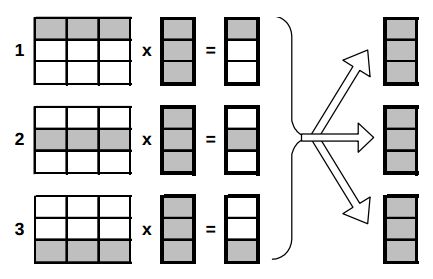
\includegraphics[width=0.5\textwidth]{illustrations/matrix-vector-product/rowwise.png}
  \caption{Computation scheme for parallel matrix-vector multiplication base on rowwise striped matrix partitioning.}
  \label{fig:rowwise-scheme}
\end{figure}


\subsubsection{Efficiency analysis} % (fold)
\label{ssub:efficienct_analysis}
Let us consider the time complexity of the algorithm of matrix-vector multiplication. If matrix $A$ is square $(m=n)$, the sequential algorithm of matix-vector multiplication has the complexity
\begin{equation}
  T_1 = n(n-1+n)\approx 2n^2 = O(n^2)
\end{equation}
In case of parallel computations each processor performs multiplication of only a part (stripe) of the matrix $A$ by the vector $b$. The size of these stripes is equal to $n/p$ rows. In case of computing the inner product of one matrix row by a vector, it is necessary to perform the $n$ multiplications and $(n-l)$ additions. Therefore, computational complexity of the parallel algorithm is determined as:
\begin{equation}
  T_p = \frac{n(n-1+n)}{p} \approx \frac{2n^2}{p} = O(\frac{n^2}{p})
\end{equation}

Taking into accoun this estimation, the criteria of speedup and efficiency of the parallel
\begin{align}
  S_p &= \frac{T_1}{T_p} = \frac{n^2}{n^2/p} = p \\
  E_p &= \frac{T_1}{pT_p} = \frac{n^2}{p(n^2/p)} = 1
\end{align}
These estimations of the computation execution time are expressed in the number of operations. Besides, they are formed \emph{without} taking into consideration the execution of data communication operations. Let us use the above mentioned assumptions that the executed multiplications and additions are of equal duration $\tau_F$.

The computation time of the parallel algorithm is
\begin{equation}
  T_p(calc) = \# rows \times \# ops/row \times \tau_F = \frac{n}{p} \cdot (2n-1) \cdot \tau_F
\end{equation}

After doing the calculations, we use MPI\_Allgather to gather all the $c$-parts on all processors. This works using a binary tree, and so the gather operation can be performed in $\log_2 p$ iterations. In the first iteration, each process sends its part (of size $n/p$) to another process, which in turn will send its own part plus the part it received (total size $2n/p$) on to the next process in the next iteration; thus, the amount of data to be sent doubles in each iteration. As a result, the all gather operation execution time when the hockney model is used can be represented as
\begin{equation}
  T_p (comm) = \sum_{i=1}^{\log_2 p} \left( \tau_S + 2^{i-1} w \frac{n}{p} \gamma \right)
  = \tau_S\log_2 p + w \frac{n}{p} \left( 2^{\log_2 p} -1 \right) \gamma
\end{equation}
where $w$ is the size of each element. The rule $\sum_{i=1}^N x^{i-1} = x^N - 1$ has been used to simplify the expression. Thus, the total time of parallel algorithm execution is
\begin{equation}
  T_p = \frac{n}{p} (2n-1) \tau_F + \tau_S \log_2 p + (p-1) w \frac{n}{p}\gamma
\end{equation}

% subsubsection efficienct_analysis (end)

Note that in this case, we end up with the complete $c$ vector on all processes.

% subsection matrix_vector_multiplication_in_case_of_rowwise_data_decomposition (end)

\subsection{Columnwise strip partitioning} % (fold)
\label{sub:matrix_vector_multiplication_in_case_of_columnwise_data_decomposition}
At the starting point of the parallel algorithm of matrix-vector multiplication each basic task $i$ carries out the multiplication of its matrix $A$ column by element $b_i$. As a result, vector $c'(i)$ (the vector of intermediate results) is obtained in each subtask. The subtasks must further exchange their intermediate data in order to obtain the elements of the result vector $c$ (element $j$, of the partial result $c'(i)$ of the subtask $i$ must be sent to the subtask $j$). This all-to-all communication or total exchange is the most general communication procedure and may be executed with the help of the function MPI\_Alltoall of MPI library. After the completion of data communications each basic subtask $i$ will contain $n$ partial values $c'_i(j)$. Element $c_i$ of the result vector $c$ is determined after the addition of the partial values (see Figure~\ref{fig:colwise}).

\begin{figure}[htbp]
  \centering
  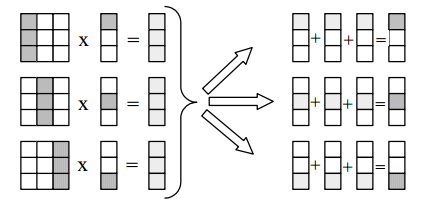
\includegraphics[width=.5\textwidth]{illustrations/matrix-vector-product/column.png}
  \caption{Computation scheme for parallel matrix-vector multiplication based on columnwise striped matrix decomposition. Note that here, we only end up with part of the (summed) $c$ vector on each process.}
  \label{fig:colwise}
\end{figure}



\subsubsection{Efficiency analysis} % (fold)
\label{ssub:efficienct_analysis}
As previously, let matrix $A$ be square, i.e. $m=n$. At the first stage of computations each processor multiplies its matrix columns by the vector $b$ elements. The obtained values are summed for each matrix row separately:
\begin{equation}
  c_s'(i) = \sum_{j=j_0}^{j_{l-1}} a_{sj}b_j, \quad 0\leq s < n
\end{equation}
where $j_0$ and $j_{l-1}$ are the initial and final column indeces of the subtasks $0\leq i <n$. As the sizes of matrix stripes and the block of the vector $b$ are equal $n/p$, the time complexity of such computations may be estimated as
\begin{equation}
  T' = \frac{n(n-1+n)}{p} \approx \frac{n^2}{p}
\end{equation}
operations. After the subtasks have exchanged the data at the second stage of computations each processor sums the obtained values up for its block of the result vector $c$. The number of the summed values for each element $c_i$ of vector $c$ conincides with the number of processors $p$. The size of result vector block is equal to $n/p$. Thus, the number of operations carried out for the second stage appears to be equal to
\begin{equation}
  T'' = \frac{n}{p} p = n
\end{equation}
Thus the total computation time is
\begin{equation}
  T_p = T' + T'' = \frac{n^2}{p} + n \approx \frac{n^2}{p}
\end{equation}
With regards to the relations obtained the speedup and the efficienct of the parallel algorithm may be expressed as follows:
\begin{equation}
  S_p = \frac{T_1}{T_p} = \frac{n^2}{n^2/p} = p, \quad E_p = \frac{T_1}{pT_p} = \frac{n^2}{p(n^2/p)} = 1
\end{equation}

Now let us consider more accurate relations for estimation of the time of parallel algorithm execution. With regard to the above discussion the execution time of the parallel algorithm computations may be estimated by means of the following expression:
\begin{equation}
  T_p (calc) = \left[ \frac{n}{p} \left(\frac{n}{p} - 1 + \frac{n}{p} \right) \cdot p + \frac{n}{p} \cdot p \right]\tau_F
   = \left[ n \left( 2 \frac{n}{p} -1 \right) + n \right] \cdot \tau_F
\end{equation}

Let us discuss two possible methods to carry out the total exchange. The first method is provided by the algorithm, according to which each processor sends its data to all the rest of computer system processors sequentially. Let us assume that the processors may simultaneously send and receive messages, and there is a direct communication line between any pair of processors. The time complexity estimation (execution time) of the total exchange algorithm may be written as follows:
\begin{equation}
  T_p^1(comm) = (p-1) \left( \tau_S + w \frac{n}{p} \gamma \right)
\end{equation}
The meaning of the terms are as follows:
\begin{itemize}\itemsep=0em
  \item $(p-1)$ -- Each processor sends data to all processors, except for self (this happens in parallel from each process).
  \item $n/p$ -- The section $c_i$ is sent to process $p_i$.
\end{itemize}

The second method of carrying out the total exchange utilizes binary distribution (in a hypercube); this could be implemented using MPI\_Allreduce with the add option. The algorithm may be executed in $\log_2 p$ steps. At each step each processor sends and receives a message of $n/2$ elements. The execution time of the data communication is then
\begin{equation}
  T_p(comm) = \log_2 p \left( \tau_S + w \frac{n}{2} \gamma \right)
\end{equation}

The two different expressions for th etotal execution time is
\begin{align}
    T_p^1 &= \left[ n \left( 2 \frac{n}{p} -1 \right) + n \right] \cdot \tau_F
           + (p-1) \left( \tau_S + w \frac{n}{p} \gamma \right)\\
    T_p^2 &= \left[ n \left( 2 \frac{n}{p} -1 \right) + n \right] \cdot \tau_F
           + \log_2 p \left( \tau_S + w \frac{n}{2} \gamma \right)
\end{align}

\emph{\textbf{Note:}} If we wanted to end up with the complete vector $c$ on all processes using the first approach, we can simply send all $n$ elements to all processes, instead of $n/p$.
% subsubsection efficienct_analysis (end)

\subsubsection{Alternative: gather the final $c$ on all processes} % (fold)
\label{ssub:alternative_gather_the_final_c}
Here we want to end up with the complete soluition $c$ on all processes. Figure~\ref{fig:rowwise-alt} illustrates this case. One way of doing this is simply doing as in $T_p^1$ above, but sending the entire vector $c$ to all processes. The other way is using MPI\_Allreduce with the summing parameter. The computation times are the same, but our two new communication times are, respectively,
\begin{align}
  T_p^1(comm) &= (p-1) \left( \tau_S + w n \gamma \right) \\
  T_p^2(comm)   &= \log_2 p \left( \tau_S + w n \gamma \right)
\end{align}

How the summing in the MPI\_Allreduce function works is illustrated in


\begin{figure}[htbp]
  \centering
  \includegraphics[]{illustrations/matrix-vector-product/columnwise.pdf}
  \caption{Columnwise partitioning. All parts $c_i$ are summed on all processors, resulting in all processes getting the complete solution $c$.}
  \label{fig:rowwise-alt}
\end{figure}

\begin{figure}[htbp]
  \centering
  \includegraphics[]{illustrations/matrix-vector-product/mpi_allreduce_sum.pdf}
  \caption{MPI\_Allreduce summing.}
  \label{fig:mpi_reduce}
\end{figure}

% subsubsection alternative_gather_the_final_c (end)
% section matrix_vector_multiplication_in_case_of_columnwise_data_decomposition (end)


\subsection{Block partitioning} % (fold)
\label{sub:block_partitioning}
$m$ is the number of matrix rows and $n$ is the number of matrix columns. These are divided into $s$ sets of rows and $q$ sets of columns; $p=sq$ blocks in total.

Let us consider the general scheme of parallel computations for matrix-vector multiplication based on checkerboard block decomposition. After multiplication of matrix blocks by blocks of the vector $b$ each subtask $(i,j)$ will contain the partial results vector $c'(i,j)$, which is determined according to the following expressions:
\begin{equation}
  c_\nu'(i,j) = \sum_{u=0}^{l-1} a_{i_\nu j_{u}} b_{j_u}, \quad i_\nu = ik+\nu, \; 0\leq \nu < k, \; k = m/s, \; j_u = jl+u, \; 0 \leq u \leq l, \; l = n/q
\end{equation}

Element by element addition of vectors of partial results for each horizontal stripe (reduction) of matrix blocks leads to obtaining the result vector $c$:
\begin{equation}
  c_\eta = \sum_{j=0}^{q-1} c_\eta ' (i,j), \quad 0\leq \eta <m, \; i=\eta /s, \nu = \eta -i s
\end{equation}

To allocate the vector $c$ we will use the same scheme that was used for the vector $b$. Let us organize the computations in such a way that after the computation termination the vector $c$ would be distributed in each of the vertical stripes of matrix blocks. Hence, each block of the vector $c$ must be duplicated on each horizontal stripe. Addition of partial results and duplicated of the result vector blocks are the necessary operations. They may be provided with the help of the fucntion MPI\_Allreduce of MPI library.

The general scheme of the performed computations for matrix-vector multiplication in case of checkerboard
block data distribution is shown in Figure~\ref{fig:blockdist}.

\begin{figure}[htbp]
  \centering
  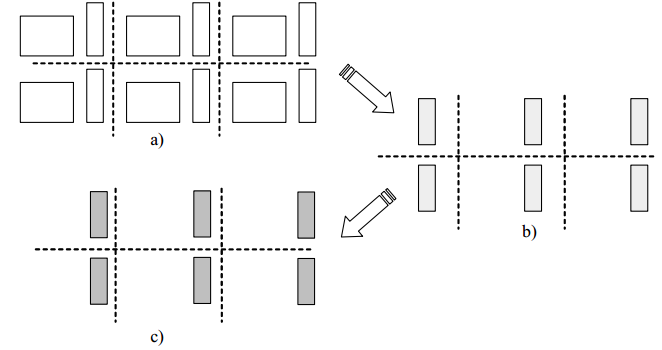
\includegraphics[width=.9\textwidth]{illustrations/matrix-vector-product/block.png}
  \caption{General scheme of parallel matrix-vector multiplication based on checkerboard block decomposition: a) the initial result of data distribution, b) the distribution of partial result vectors, $c$) the block distribution of result vector $c$}
  \label{fig:blockdist}
\end{figure}

On the basis of analysis of this parallel computation scheme it is possible to draw the conclusion that the information dependencies of the basic subtasks appears only at the stage of summing the results of multiplication of matrix blocks by blocks of the vector $c$. These computations may be performed according to the cascade scheme (see Section 2). As a result, the structure of the available information communications for the subtasks of the same horizontal block stripe corresponds to the topology of the binary tree.
% subsection block_partitioning (end)

\subsubsection{Scaling and Distributing Subtasks among Processors} % (fold)
\label{ssub:scaling_and_distributing_subtasks_among_processors}
The size of matrix blocks may be chosen in such a way that the total number of the basic subtasks would
coincide with the number of processors $p$. Thus, for instance, if the size of the block grid is defined as $p=s\cdot q$, then
\[
  k = \frac{m}{s}, \quad l = \frac{n}{q}
\]
where $k$ and $l$ are the number of rows and columns in matrix blocks. This method of defining the block sizes makes the amount of computations in each subtask be the same. Hence, complete balance of computational load among processors is achieved.

Choice is also possible in defining the sizes of matrix block structure. A great number of horizontal blocks leads to the increase of the number of iterations in the reduction of block multiplication results. The increase of the vertical size of the block grid enhances the amount of the data transmitted among the processors. The simple frequently used solution consists in the use of the same number of blocks both vertically and horizontally, i.e.
\[
  s = q = \sqrt{p}
\]

It should be noted, that the checkerboard block scheme of data decomposition can be considered as the generalization of all the approaches discussed in this Section. Actually, if $q=1$ the block grid is reduced to the set of horizontal stripes, if $s=1$ the matrix $A$ is partitioned into the set of vertical stripes.

The possibility to carry out data reduction efficiently must be taken into account in solving the problem of distributing subtasks among the processors. A suitable approach may consist in distributing the subtasks of the same horizontal stripes among processors for which the network topology is a hypercube or a complete graph.
% subsubsection scaling_and_distributing_subtasks_among_processors (end)


\subsubsection{Efficiency analysis} % (fold)
\label{ssub:efficiency_analysis}
Let us carry out the efficiency analysis for the parallel matrix-vector multiplication algorithm making the usual
assumptions that matrix $A$ is square, i.e. $m=n$. We will also assume that the network topology is rectangular grid
$p=s\cdot q$ ($s$ is the number of rows in the processor grid and $q$ is the number of columns).

The general efficiency analysis leads to ideal parallel algorithm characteristics:
\begin{equation}
  S_p = \frac{n^2}{n^2/p}, \quad E_p = \frac{n^2}{p(n^2/p)}
\end{equation}

To make the obtained relations more precise we will estimate more exactly the number of algorithm
computational operations and take into account the overhead related with data communications among the
processors.

The total time of multiplication of matrix blocks by the vector $b$ may be evaluated as follows:
\begin{equation}
  T_p(calc) = \frac{n}{s} \cdot \left( 2 \frac{n}{q} - 1 \right) \tau_F
\end{equation}

Data reduction may be performed with the use of the cascade scheme. Thus, it includes $\log_2 q$ iterations of transmitting messages of $w \frac{n}{s}$ size. As a result, the estimation of communication overhead in accordance with the Hockney model may be evaluated by means of the following expression:
\begin{equation}
  T_p(comm) = \log_2 q \left( \tau_S + w \frac{n}{s} \gamma \right)
\end{equation}

The meaning of the different terms is as follows:
\begin{itemize}\itemsep=0em
  \item $\log_2 q$ -- $q$ columns bay be summed in $\log_2 q$ steps.
  \item $n/s$ -- Each column contains $n/s$ rows.
\end{itemize}

Thus, the total time of carrying out parallel algorithm of matrix-vector multiplication based on checkerboard block
decomposition is the following:
\begin{equation}
  T_p = \frac{n}{s} \cdot \left( 2 \frac{n}{q} - 1 \right) \tau_F + \log_2 q \left( \tau_S + w \frac{n}{s} \gamma \right)
\end{equation}

Note that at the end of this, each grid row only contains the part of $c$ corresponding on the part of $b$ that was on the row. We can gather this at the end in $O(\log_2 s)$ time with an MPI\_Allgather call.


% subsubsection efficiency_analysis (end)


\subsection{Summary} % (fold)
\label{sub:summary}
For small $n$, block-partitioning is significantly slower than the other two because of more communication. However, it allows for more partitioning of the data and can thus allow us so solve larger systems.

Rows are better for OpenMP: less data transfer, better to let each thread do more on each row than do many small rows

% subsection summary (end)




% section matrix_multiplication (end)
